
\chapter{Linkage and the canonical sheaves of singular curves}
\label{LiaisonChapter}\label{linkageChapter}\label{LinkageChapter}


\section{Introduction} \label{LinkageIntro}

\emph{In this chapter, curves are purely \1-dimensional projective
schemes, 
not always
reduced or irreducible.}

Linkage is an equivalence relation on varieties and schemes of a given
dimension embedded in a common space. It was a key element
in the classification of curves in $\PP^3$ for which
Max Noether and Georges-Henri Halphen
\index{Noether @Noether, Max}%
\index{Halphen, Georges-Henri}%
received the
Steiner prize
\index{Steiner prize}%
of the Prussian
Academy of Sciences in 1880, and it was a necessary ingredient in the
work of
Clebsch, Brill, Noether and Macaulay
toward
\index{Clebsch @Clebsch, Rudolf Friedrich Alfred}%
\index{Brill @Brill, Alexander}%
\index{Macaulay @Macaulay, Francis Sowerby}%
\index{Riemann--Roch theorem}%
a version of the
Riemann--Roch theorem
couched in terms of the algebra
of plane curves near the end of the nineteenth century.
It was put on a firm modern footing in \cite{MR364271}, and this
\index{Hartshorne @Hartshorne, Robin}%
\index{Prabhakar Rao, A.}%
\index{Rao, A. Prabhakar}%
\index{Peskine @Peskine, Christian}%
\index{Szpiro @Szpiro, Lucien}%
foundation was used for further progress in projective geometry by
Hartshorne, Rao
and others. In this chapter we will explain some of
these developments, starting with a simple example,
\index{historical context}%
and including the algebra necessary for a formulation in the natural
generality of purely 1-dimensional schemes.

As we have seen, any plane curve is
arithmetically Cohen--Macaulay,
\index{ACM}%
and
its arithmetic genus is determined by its degree. Similarly, a curve in
$\PP^3$ that is a 
complete intersection
\index{complete intersection}%
of surfaces of degrees $d,e$
is arithmetically Cohen--Macaulay (Theorem~\ref{Lasker}) and has
arithmetic genus determined by $d,e$.
Next simplest, perhaps,
\index{directly linked}%
is a curve $C$ that is
\emph{directly linked}
to a complete intersection,
which means roughly that its union $X = C\cup D$
with a complete intersection
curve $D$ is again a complete intersection
(see Definition~\ref{linkage def} for the general definition).
We will see that, once again, such a
curve $C$ is arithmetically Cohen--Macaulay,
and its genus is determined by the degrees of the equations of $X$
and the degree and genus of $D$.
Allowing sequences of direct links we define an equivalence relation
\index{linkage|(}%
\index{licci}%
called  \emph{linkage} or \emph{liaison},
and curves in the \underline{li}nkage {\underline c}lass of a {\underline
c}omplete {\underline i}ntersection are
said to be
\emph{licci}.

A famous theorem of Hartshorne and Rao \cite{MR520926} shows that the
linkage class of a curve $C\subset \PP^3$
is classified by the finite-dimensional graded module
$$
D(C) \colonequals H^1_*(\sI_C)\colonequals \bigoplus_{m\in \ZZ}
H^1(\sI_C(m)),
$$
called the
\emph{deficiency module} or \emph{Hartshorne--Rao module}
\index{deficiency module}%
\index{Hartshorne--Rao module}%
of $C$. (This is a module over the
homogeneous coordinate ring $S = H^0_*(\cO_{\PP^3})$.) The correspondence
is explicit: from a finite-dimensional graded module over $S$ one can
actually construct curves.

In the first sections of this chapter we will examine the equivalence
relation on curves in $\PP^3$ that is defined by linkage. Much of the
story extends to the case of singular curves. This extension requires
an understanding of the dualizing sheaves of singular curves, to which
we turn in
\index{dualizing sheaf}%
Section~\ref{duality}. We conclude the chapter with an analysis of the
adjoint ideal, completing a result from
\null Chapter~\ref{PlaneCurvesChapter},
and allowing us to formulate
the Riemann--Roch theorem for general curves and coherent sheaves.

Aside from the classification result above, linkage is useful in analyzing
Hilbert schemes.
We will exploit this systematically in cases of low
degree and genera in Chapter~\ref{HilbertSchemesChapter}, and we begin
this chapter with what is perhaps the simplest example, computing the
dimension of the component of
\index{Hilbert scheme}%
the Hilbert scheme $\Hilb_{3m+1}(\PP^3)$ that is the closure of
the open subset $\cH^\circ$  parametrizing twisted cubics (see
Proposition~\ref{hilb of twisted cubics} for another proof).

\section{Linkage of twisted cubics}
The simplest example of linkage is that of the union of a
\index{twisted cubic!linkage of}%
twisted cubic and one of its secant lines, pictured in
Figure~\ref{cubicAndLine}, and we will start with that.

\begin{figure}
\fboxsep=0pt
\fbox{\includegraphics[height=3in]{"main/Fig15-1-TwistAndShout"}}
\caption{A quadratic cone (red) intersecting a smooth quadric (yellow) in
the union of a vertical line and a twisted cubic (credit: Herwig Hauser).}
\label{cubicAndLine}
\end{figure}

Any twisted cubic curve $C\subset \PP^{3}$ lies on a nonsingular quadric
in class $(1,2)$. Adding a line $L$ of class
$(1,0)$ we get a  divisor of class $(2,2)$, the class of the complete
intersection of two quadrics. Since $L$ is also
a complete intersection, $C$ is licci.

We can make the relation of $L$ and $C$ explicit as follows: The ideal
of $C$
is minimally generated by the three $2\times 2$ minors of the matrix
$$
\begin{pmatrix}
x_0&x_1&x_2\\
x_1&x_2&x_3
\end{pmatrix}\,.
$$
The minor $Q_{1,2}$ involving the first two columns and the minor
$Q_{2,3}$ involving the last two columns
both vanish on the line $L: x_1 = x_2 = 0$, which meets the twisted
cubic in the two points
$x_{0}= x_{1}=x_{2}=0$ and $x_{1} = x_{2} = x_{3}= 0$. Thus $L$ is a
secant line to $C$.
A general linear combination $Q$ of $Q_{1,2}$ and $Q_{2,3}$ defines
a smooth quadric, which is thus isomorphic to $\PP^1\times \PP^1`
`$. The curve $C$ necessarily lies in the divisor class $(1,2)$ (or,
symmetrically, $(2,1)$), and the line in class $(1,0)$ (respectively,
$(0,1)$), summing to the
\index{complete intersection!of two quadrics}%
complete intersection $(2,2)$ of Q with (say) $Q_{1,2}$. See
Figure~\ref{cubicAndLine}.

Conversely, if two irreducible quadrics $Q_{1}, Q_{2}$ both contain a
twisted cubic $C$ then, by
B\'ezout's theorem,
\index{Bezout@B\'ezout's theorem}%
$Q_{1}\cap Q_{2}$ is the union of $C$ with a line. If at least one of
the quadrics is smooth, we are in the
situation above.

This suggests that we set up an incidence correspondence between twisted
cubics and their secant lines. Let $\PP^9$ denote the projective space
of quadrics in $\PP^3` `$, and consider
$$
\Phi = \bigl\{@ (C, L, Q, Q') \in \cH^\circ \times \GG(1,3) \times \PP^9 \times
\PP^9 \, \mid \, Q \cap Q' = C \cup L@ \bigr\}.
$$
We'll analyze $\Phi$ by considering the projection maps to $\cH^\circ$
and $\GG(1,3)$; that is, by looking at the diagram
$$\small\xymatrix{
 &  \Phi \ar[rd]^{\pi_2}\ar[ld]_{\pi_1} & \\
\cH^\circ & & \GG(1,3)
}
$$

Consider  the projection map $\pi_2 : \Phi \to \GG(1,3)$ on the second
factor. By what we just said, the fiber over any point $L \in \GG(1,3)$
is an open subset of $\PP^6 \times \PP^6` `$, where $\PP^6$ is the space
of quadrics containing $L$. Since $\dim \GG(1,3) = 4$ we see that $\Phi$
is irreducible of dimension $4 + 2\times 6 = 16$. On the other hand,
the map $\pi_1 : \Phi \to \cH^\circ$ is surjective, with fiber over a
curve $C$ an open subset of $\PP^2 \times \PP^2` `$, where $\PP^{2}$
is the projective space of quadrics containing $C$; we conclude that
$\cH^\circ$ is irreducible of dimension 12, in accord with our
computation in Proposition~\ref{hilb of twisted cubics} of the space of
twisted cubics as
$\PGL_4/` `\PGL_2$.
\index{PGL@$\PGL_4/` `\PGL_2$}%


\section{Linkage of smooth curves in $\PP^3$}
\label{SLinkage}\label{linkage section}

If the union of two smooth curves in $\PP^3$ is a 
complete intersection
\index{complete intersection}%
then the degrees and genera
of the curves are related:

\begin{theorem}\label{liaison genus formula-first version}
Let $C_1, C_2\subset \PP^3$ be distinct smooth irreducible curves
whose union is the complete
intersection
of two surfaces $S,T$
of degrees $s,t$,
with $S$ smooth.
Then $ \deg C_1+\deg C_2 = st$ and
$$
g(C_1) - g(C_2) = \frac{s+t-4}{2}(\deg C_1-\deg C_2).
$$
\end{theorem}

In words, the difference between the genera of $C_1$ and $C_2$
is proportional to the difference in their degrees, with constant of
proportionality $(s+t-4)/2$.
In the
example of a
complete
intersection of two quadrics
described above, the multiplier $(s+t-4)/2$
is zero,
and indeed the line
and the twisted cubic have the same genus.
The relation of degrees and genera is true more generally, as we shall
see in the next section, but the special
case is already useful.

\begin{proof}
The sum of degrees of $C_1$ and $C_2$ is the degree of $ C_1\cup C_2=S\cap T$,
which, by B\'ezout's theorem, is $st$.

By the
adjunction formula
\index{adjunction formula}%
in $\PP^3$ the
canonical divisor
of $S$ has
\index{canonical divisor}%
\index{Bezout@B\'ezout's theorem}%
class $K_S = (s-4)H$. Thus, from the
adjunction formula on the surface $S$ we get
$$
g(C_i) = \frac{C_i^2+C_i\cdot K_S}{2}+1 = \frac{C_i^2+(s-4) \deg
C_i}{2}+1.
$$
Subtracting,
$$
g(C_1)-g(C_2) = \frac{C_1^2-C_2^2+(s-4) (\deg C_1-\deg C_2)} {2}.
$$
Because $C_1+C_2$ is in the class $tH$ on $S$ we have
$$
C_1^2-C_2^2 = (C_1+C_2)(C_1-C_2) = t(\deg C_1-\deg C_2).
$$
Combining the last two displays yields
the second formula
of the theorem.
\end{proof}


\begin{remark}
Linkage is closely related to linear equivalence.
\index{linear equivalence}%
Here is a special case:
suppose that $S$ is a smooth surface in $\PP^3` `$, and $C\subset S$
is a curve. If $T$ is a sufficiently general surface of degree $t$
containing $C$ then the curve $C'$ that is the link of $C$ with respect
to $S,T$ lies in the class $tH-C$. If we link again with
respect to another surface $T'$ of degree $t'$ we thus arrive at $C''
= C+(t-t')H$. Thus if $t=t'$ we get a curve in the same
linear equivalence class as $C$. Moreover, since every rational function
on $S$ is the restriction to $S$ of the ratio of two forms of the same
degree on $\PP^3` `$,
the set of curves on $S$ that can be obtained from $C$ by two linkages
with surfaces $T, T'$ of the same degree is exactly the
linear series $|C|$ on~$S$. This idea is generalized in the notion of
a \emph{basic double link}; see
\index{basic double link}%
Exercise~\ref{Basic double links}.
\end{remark}

\section{Linkage of purely 1-dimensional schemes in $\PP^3$}
To say that the union $X$ of distinct reduced irreducible curves $C\cup C'$
is a complete intersection means that
the ideal $I_X $
equals
$I_C\cap I_{C'}$. Since
the latter
contains
$I_CI_{C'}$, the ideal quotient
$(I_X:I_C) := \{F \mid FI_C\subset I_X\}$
contains $I_{C'}$.

On the other hand, if $F \notin I_{C'}$ and we choose $G\in I_C\setminus
I_{C'}$, then $FG\notin I_{C'}$, so
$F\notin (I_X:I_C)$, and thus
$(I_X:I_C) = I_{C'}$.
This
relationship
underlies
the formulas connecting the degrees and genera of $C,C'$, which hold
for arbitrary purely 1-dimensional subschemes of $\PP^3` `$, as we shall see in Theorem~\ref{direct linkage}.

\begin{definition}\label{linkage def}
Let $C,C'$ be purely \1-dimensional subschemes of $\PP^3` `$. We say that
$C'$ is \emph{directly linked} to $C$ if there is a complete
intersection $X$ containing $C,C'$ and
satisfying
$(I_X:I_C) = I_{C'}$. We say that
$C'$ is \emph{linked} to $C$ if they are connected by a chain of such
\index{linked, evenly linked|defi}%
\index{evenly linked|defi}%
direct linkages, and we say that $C'$ is \emph{evenly linked} to $C$
if the chain involves an even number of direct linkages.
\unif
\end{definition}

Note that in this setting, $C$ and $C'$ can have components in
common. For example, the subscheme $C \subset
\PP^3$ defined by the square of the ideal $\cI_{L/\PP^3}$ of a line $L
\subset \PP^3$ is linked to the reduced line $L$ in the complete
intersection of two quadrics.
This makes sense, since $C$ is a
flat limit of twisted cubics.
$C$ is an example of a rope; see
\index{rope}%
Exercise~\ref{line and rope} for more.

As in the smooth case treated above, direct linkage is a symmetric
relation:

\begin{proposition}\label{link unmixed}
Let $C_1\subset \PP^3$ be a purely \1-dimensional subscheme with saturated
\index{saturated ideal}%
homogeneous ideal $I_1$ and suppose that $C_1$ is contained in a complete
intersection of
hypersurfaces $X \colonequals  S\cap T$. The ideal $I_2 = (I_{X}:I_1)$
is a saturated ideal, defining a purely \1-dimensional subscheme and
$I_1 = (I_{X}: I_2)$ as well.
\unif
\end{proposition}

\begin{proof}
The ideal $I_{X}$ is unmixed of
\index{unmixed ideal}%
codimension 2, since $X$ is a complete intersection
\cite[Proposition 18.13]{Eisenbud1995}. It follows
that $I_2 = (I_{X}:I_1)$
is also unmixed of codimension 2,
and therefore
saturated.
Thus it suffices to prove that $I_1 = (I_{X}: I_2)$ after localizing at
a codimension 2 prime $P$
that contains $I_{X}$.

Write $R$ for the localization at $P$ of the homogeneous coordinate ring
of~$X$.
Because $I_{X}$ is a complete intersection, the ring $R$
is zero-dimensional and
Gorenstein.
\index{Gorenstein}%
By \cite[Propositions 21.1 and 21.5]{Eisenbud1995}, every finitely
\index{reflexive}%
generated $R$-module is
reflexive.
Since
$I_{C_2}R= \ann_{R}(I_{C_1}R) \cong \Hom_R(R/I_{C_1}R, R)$,
the proposition follows.
\end{proof}

\section{Degree and genus of linked curves}
\label{duality} % resolves to section number

The degrees and
arithmetic genera
\index{arithmetic genus}%
of directly linked schemes are related \null exactly as in the
pilot case of Section~\ref{SLinkage}.

\begin{theorem}\label{direct linkage}\label{linked genus formula}
If $C_1,C_2\subset \PP^3$ are purely $1$-dimensional schemes that are
directly linked by surfaces $S,T$ of degrees $s,t$, then
$\deg C_1+\deg C_2 = st$ and
\vspace*{3pt}
$$
p_a(C_1) - p_a(C_2) = \frac{s+t-4}{2}(\deg C_1-\deg C_2).
$$
\end{theorem}

Since we have left the realm of smooth curves and surfaces, we will need
a more sophisticated
duality theory,
\index{duality}%
and we
postpone the proof to explain the necessary ideas.

\subsection*{Dualizing sheaves for singular curves}

In Chapter~\ref{RiemannRochChapter} we said that the
canonical sheaf of a smooth curve\emdash the sheaf of differential
forms\emdash was the most important invertible sheaf after the
structure sheaf. In the general setting of Cohen--Macaulay schemes,
the analogue of the canonical sheaf is
known as
the dualizing sheaf.
The general definition of
the dualizing sheaf of a pure-dimensional projective scheme
is not very illuminating;
what is useful is how it is constructed and its cohomological properties
relating to duality.
However, having a definition may be comforting.

\begin{definition}
Let $X$ be a projective scheme  of pure dimension $d$ over $\CC$. The
\index{dualizing sheaf}%
\emph{dualizing sheaf} for $X$ is a coherent sheaf $\omega_X$
\label{dualizing sheaf for singular curve}
together
with a \emph{residue map} $\eta: H^d(\omega_X) \to\nobreak \CC$ such that for
\index{residue!map}%
every coherent sheaf  $\sF$ the composite map
$$
H^d(\sF) \times \Hom(\sF, \omega_X) \to H^d(\omega_X) \ruto {\ \eta} \CC
$$
is a
perfect pairing.
\index{perfect pairing}%
\unif
\end{definition}

If $\cF = \sL$ is an invertible sheaf on a projective curve $C$
then $\Hom(\sL, \omega_X) = \sL^{-1}\otimes \omega$,
so
we recover
Serre duality:
\index{Serre duality}%
$H^{1}(\sL)$ is the dual of
$H^{0}(\sL^{-1}\otimes \omega_{C})$.

It follows from the definition that the pair $(\omega_{X}, \eta)$ is
unique up to canonical isomorphism if it exists:
The module $H^{0}_{*}(\omega_{X}) = \bigoplus_{n\in \ZZ}(\Hom_{X}(\sO_{X}(n),
\omega_{X}))$
is determined as the graded vector space dual of $H^{d}_{*}(\sO_{X})$,
and the choice of $\eta$ simply fixes the isomorphism. It may not be
apparent that such a sheaf exists, but we will give a construction in
Section~\ref{dualizing sheaves section}.

Several properties of the dualizing sheaf on a purely 1-dimensional
scheme
are the same as in the smooth case, and follow easily from the definition:

\begin{proposition}\label{similarities}
Let $C$ be
a purely \1-dimensional projective scheme.
\begin{enumerate}

\item $\sHom_C(\omega_C, \omega_C) = \sO_C$; thus if $C$ is integral
then the generic rank of $\omega_C$ is \1.

\item For any invertible sheaf $\sL$ on $C$ we have
$$H^1(\sL^{-1})= H^0(\sL\otimes \omega_{C})\quad \hbox{and} \quad
H^0(\sL^{-1} ) = H^1(\sL\otimes \omega_{C}).
$$
In particular,
$\chi(\sL^{-1}) = -\chi(\sL\otimes \omega_{C})$.
\end{enumerate}
\end{proposition}

\begin{proof}
(1)\, We
will show
that the natural map $\sO_C \to
\sHom_C(\omega_C, \omega_C)$ is an isomorphism.
Since the map is globally defined, it suffices to prove that it is an
isomorphism locally.

Choose a
Noether normalization
\index{Noether normalization}%
of $C$, that is, a finite map $f: C\to \PP^1` `$.
We shall see in Theorem~\ref{canonical as Hom} below that $\omega_C \cong
\sHom_{\PP^1}(\sO_C,\omega_{\PP^1})$, regarded as a sheaf on $C$ (in
Theorem~\ref{canonical as Hom} this is the sheaf $f^{!}\omega_{\PP^{1}}$).
Since $C$ is purely 1-dimensional, $\sO_{C}$ is torsion-free as an
$\sO_{\PP^{1}}$-module, and is thus locally
free.
Also, since $\PP^{1}$ is smooth, $\omega_{\PP^{1}}$ is locally
isomorphic to $\sO_{\PP^{1}}$.
But if $B$ is any commutative ring and $A$ is a $B$-algebra that is
finitely generated and free as a $B$-module, then the composite map
$$
A \to \Hom_{A}(\Hom_B(A,B),\Hom_B(A,B)) \cong \Hom_{B}(\Hom_B(A,B), B)
$$
sending an element $a$ to the multiplication by $a$ and thence to the
map $f\mapsto f(a)$
may be identified with the isomorphism of $A$ to
its double dual as a $B$-module;
this completes the argument.
(See Exercise~\ref{adjointness} for a
generalization of this last step.)

\noindent(2)\, The definition of $\omega_C$ shows that, if $\sL$
is an invertible sheaf, then
$$
H^1(\sL^{-1}) = \Hom_C(\sL^{-1}, \omega_C))
= H^0(\sHom_C(\sL^{-1}, \omega_C))
= H^0(\sL\otimes_C \omega_{C}).
$$
Using part (1), we have
$$\let\\\cr
\eqalignbot{
H^0 (\sL^{-1})
&= H^0 (\sL^{-1}\otimes_{C}\sO_{C})\\
&= H^0 \bigl(\sL^{-1}\otimes_{C}\sHom_C(\omega_{C}, \omega_{C})\bigr) \\
&= \Hom_{C}(\sL\otimes_C \omega_{C},  \omega_{C}))\\
&= H^{1}(\sL\otimes_{C}\omega_{C})
}
\eqno\qedhere
$$
\end{proof}


\section{The construction of dualizing sheaves}
\label{dualizing sheaves section}

Dualizing sheaves do exist on any purely 1-dimensional projective scheme, 
and more generally on any projective Cohen--Macaulay scheme. We
have already seen constructions
in three
cases:

\begin{itemize}
\item If $X$ is a smooth scheme of dimension $d$ over $\CC$ then
$\omega_{X}= \mwedge^{d} \Omega_{X/\CC}$
is a dualizing sheaf
\index{dualizing sheaf}%
[\citeNP[Section III.7]{Hartshorne1977};
\citeyear[p.~648, 708]{Griffiths-Harris1978}].
\item If $f: X\to Y$ is a map of smooth curves, then $\omega_{X} =
f^{*}(\omega_{Y})(\ram_{X/Y})$, where
$\ram$ denotes the
ramification divisor.
\index{ramification!divisor}%
\item If $X\subset Y$ is a
Cartier divisor
\index{Cartier divisor}%
on a surface, then $\omega_{X}
= \omega_{Y}(X)|_{X}$.
\end{itemize}

How can such different looking formulas all be correct?
Grothendieck
\index{Grothendieck @Grothendieck, Alexander}%
provided a general scheme
that unifies them and gives many more.
To understand what is needed for the general case, we first consider a
setting generalizing
Hurwitz's theorem.
\index{Hurwitz's theorem}%
Suppose that $X\to Y$ is a
finite map
\index{finite map}%
of projective schemes, and that
$\sF$ is a coherent sheaf on $X$.

If we restrict ourselves to open affine subsets
$U \colonequals \Spec A\subset X$ mapping to
$V\colonequals \Spec B\subset Y$ via the map of rings $f^{*}:B\to A$, then
\index{*@$*$ superscript ($f^*$)}%
$F \colonequals \sF_{U}$ is an $A$-module. Moreover,
$f_*{F} \colonequals f_*(\sF)(V)$ is just $F$ regarded as a $B$-module
via the map $f^{*}$.

For any $B$-module $M$ the module $\Hom_{B}(A, M)$ has a natural
$A$-module structure,
where $(a\phi)(m)$ is defined to be $\phi(am)$. The functor
\index{"!@"! superscript ($f^"!$)}%
$$
f^!(-)\colonequals\Hom_{B}(A,-):\operatorname{mod}_B\to\operatorname{mod}_A
$$
defined in this way is the
\index{right adjoint}%
right adjoint of the functor
$f_{*}(-):\operatorname{mod}_{A}\to \operatorname{mod}_{B}$,
which means that there is a natural isomorphism of functors
\index{*@$*$ subscript ($f_*$)}%
$$
\Hom_{B}(f_{*}F, -) \cong \Hom_{A}(F, \Hom_{B}(A, -)) = \Hom_{A}(F, f^{!}(-)).
$$
Thus
if $Y$ has dualizing sheaf $\omega_Y$ and we set
$o_Y \colonequals \omega_Y(V)$, then
$$
\Hom_{B}(f_{*}F, o_{Y}) \cong \Hom_{A}(F, f^{!}o_{Y}).
$$
Also, there is a natural transformation $\eta$ from $ f_{*}f^{!}$ to
the identity functor given by the formula
$$
\eta: f_{*}f^{!}(M) = f_{*}(\Hom_{B}, (A,M)) = \Hom_{B}, (A,M) \to M,
\quad\eta(\phi) = \phi(1),
$$
for any $A$-module $M$.
The transformation $\eta$ called the
\index{counit}%
\index{adjoint pair of functors}%
\emph{counit} of the adjoint pair
$(f_{*}, f^{!})$.

We also write $f^{!}(-)$ for the sheafification of the functor
$\Hom_{B}(A,-)$. Again $f^{!}$ is right adjoint to $f_{*}$ on coherent
sheaves,
and again there are natural maps $\eta:f_{*}f^{!}(\sF) \to\sF$.

\begin{theorem}\label{canonical as Hom}
\!Let $f{:}X{\to}Y$ be a finite map of $d$-dimensional projective schemes.
If $Y$ has a dualizing sheaf $\omega_{Y}$,
with residue map $\eta_{Y}: H^{d}(\omega_{Y}) \to \CC$,
then
$$
\omega_{X} \colonequals f^{!}\omega_{Y},
$$
with residue map
$$
\rho^{}_{X}: H^{d}(f^{!}\omega_{X}) = H^{d}(f_{*}f^{!}\omega_{X}) \,\ruuto
{\!\!H^{d}(\eta)} H^{d}(\omega_{Y}) \ruto {\!\rho^{}_{Y}} \CC,
$$
where $\eta$ is the counit of the adjoint pair $(f_{*},f^{!})$, is a
dualizing sheaf on $X$.
\unif
\end{theorem}

\begin{proof}
Let $\sF$ be a coherent sheaf on $X$. Since $f$ is finite,
$H^{d}(\sF) = H^{d}(f_{*}(\sF))$. Thus,
since $f^{!}(-)$ is a right adjoint of $f_{*}$ there are natural
isomorphisms
$$
H^{d}(\sF) = H^{d}(f_{*}\sF)
\cong
\Hom_{Y}(f_{*}\sF, \omega_{Y})^{\vee} \cong
\Hom_{X}(\sF, f^{!}\omega_{Y})^{\vee},
$$
the first being
induced by $\rho^{}_{Y}$. One
can check that the composite
isomorphism is the one induced by $\rho^{}_{X}$, so $\omega_X =
f^{!}(\omega_{Y})$, completing the proof.
\end{proof}

\begin{fact}
Given this theorem, it seems natural to look for an adjoint functor
$f^{!}$ for a wider class of morphisms
$f$, but\dots\ in most cases, for example when $f$ is the inclusion of a
divisor on a smooth surface, no such functor exists on the category of
coherent sheaves!
An adjoint functor
$f^{!}$ does exist on the derived category, where it is the right adjoint
to $Rf_{*}$, leading to a theory
of dualizing complexes.

Fortunately for the reader who is mostly interested in curves, this
level of
complication is unnecessary, and there is an intermediate level of
generality that suffices
for all the purposes of this book and more:

\begin{theorem}\label{general adjunction}
Suppose that $f: X\to Y$ is a finite map of projective schemes. If $Y$ is
Gorenstein
\index{Gorenstein}%
with
dualizing module
\index{dualizing module}%
$\omega_{Y}$, then
$$
f^{!}(\omega_{Y}) \cong \sExt^{\dim Y-\dim X}_{Y}(\sO_{X}, \omega_{Y})
$$
is a dualizing module for $X$.
\end{theorem}

The hypothesis is satisfied for any $Y$ that is smooth, or even 
locally a complete intersection.
\index{complete intersection!local}%
The
reason this works is that the complex
$f^{!} \omega_{Y}$
can be identified with its one nonvanishing cohomology module,
$\sExt^{\dim Y-\dim X}_{Y}(\sO_{X}, \omega_{Y})$.
See for example \cite{AltmanKleiman} for a thorough and accessible
exposition and the website \cite{SixOperations} for an extensive
list of further references. 
\end{fact}

\begin{proof}[Proof of Theorem~\ref{direct linkage}]
Let $X$ be the complete intersection of surfaces of degrees $s,t$
containing $C$, and let $R_X = S/(F,G)$ be its homogeneous coordinate
ring, where
$S = \CC[x_0,\dots,x_3]$ is the homogeneous coordinate ring of $\PP^3` `$.
From the free resolution
$$
\def\ruuto#1{\mathrel{\hbox{$-\mskip-8mu-\mskip-8mu-\mskip-8mu\to$}\kern-24.5pt
\raise9pt\hbox{$\scriptstyle#1$}\kern3pt}}
0\to S(-s-t) \ruuto {\tbinom{G}{-F}}
S(-s)\oplus S(-t) \ruuto {\!(F\ G)}
S \to R_{X} \to 0
$$
and Theorem~\ref{general adjunction} we see that
$$
\omega_X = \sExt^2_C(\sO_X, \omega_{\PP^3}) =\sExt^2(\sO_X,
\sO_{\PP^3}(-4)) = \sO_X(s+t-4).
$$
Note that for any ideals $J\subset I$ in a ring $A$ we have $\Hom_A(A/I,
A/J) \cong (J:I)/J$, where the isomorphism
sends a homomorphism $\phi$ to the element $\phi(1)$. From
Theorem~\ref{general adjunction} we have
\vspace*{3pt}
$$
\vspace*{3pt}
\omega_C = \sHom_X(\sO_C, \omega_X) = \sHom_X(\sO_C, \sO_X)(s+t-4) =
\frac{\sI_X:\sI_C}{\sI_X}(s+t-4),
$$
where we have identified $\sO_C$ with its pushforward under the inclusion
map $C\to X$.

By Proposition~\ref{similarities}
we have
$\chi(\omega_C(m)) = -\chi(\sO_C(-m))$. It follows that the leading
coefficient of the Hilbert polynomial of $\omega_C$
is
equal to $\deg C$, and thus
$$
st = \deg \sO_X = \deg \sO_{C'}+\deg \sO_C,
$$
as required by the formula for the sum of the degrees.

From Theorem~\ref{canonical as Hom} (or Theorem~\ref{general
adjunction}) we see that $\chi(\sO_X) = st(4-s-t)/2$. Since $\sO_{C'}
= \sO_{\PP^3}/(\sI_X : \sI_C)$ and
$(\sI_X : \sI_C)/(\sI_X) = \omega_C(4-s-t)$ we have
$$
\medmuskip2mu
\begin{aligned}
\frac{4-s-t}{2}(\deg C+\deg C')
&=\frac{4-s-t}{2}st\\
&=\chi(\sO_X) \\
&= \chi(\sO_{C'})+\chi(\omega_C(4-s-t)) \\
&= \chi(\sO_{C'})-\chi(\sO_C(s+t-4)) \\&= \chi(\sO_{C'})-(s+t-4)\deg
C-\chi(\sO_C)\\
&= (1-p_a(\sO_{C'})) - (1-p_a(\sO_C)) -(s+t-4)\deg C,
\end{aligned}
$$
whence
$$
p_a(\sO_C) -p_a(\sO_{C'}) = \frac{s+t-4}{2} (\deg C - \deg C').
\eqno\qedhere
$$
\end{proof}

Linkage also behaves in a simple way with respect to deficiency modules:

\begin{theorem}\label{HR}
If $C,C'$ are purely \1-dimensional subschemes of $\PP^3$ that are directly
linked by a complete intersection of degrees $s,t$ then
$$
D(C') = \Hom_\CC(D(C), \CC) (-s-t+4)
$$
as graded modules over the homogeneous coordinate ring of $\PP^3` `$.
\unif
\end{theorem}

A more general form of this result appears as Proposition 2.5 in
\cite{MR364271},
with an attribution to
Daniel Ferrand.
\index{Ferrand @Ferrand, Daniel}%

\begin{proof}
Suppose that the homogeneous ideal of $C$ is generated by forms of degree
$a_i$, $i=1,\dots,s$. Since $C$ is
locally Cohen--Macaulay,
\index{locally Cohen--Macaulay}%
the local rings $\sO_{C,p}$ have projective dimension 2 as modules over
$\sO_{\PP^3, p}$, and $\sI_{C,p}$ has projective dimension 1.
Thus we have an exact sequence
$$
0\to \sE \to \tsty\bigoplus\limits_i\sO_{\PP^3}(-a_i) \to \sI_C \to 0.
$$
Since the first and second cohomology groups of the twists of
$\sO_{\PP^3}$ vanish, we deduce an isomorphism
$$
\tsty
D(C) \colonequals \bigoplus\limits_{m\in \ZZ}
H^1(\sI_C(m)) \cong \bigoplus\limits_{m\in \ZZ} H^2(\sE(m)).
$$

Let $X$ be the
complete intersection of two hypersurfaces, 
of degrees
\index{complete intersection!of two surfaces in $\PP^3$}%
$s,t$, containing $C$. From the inclusion we deduce a
map of resolutions
$$
\medmuskip2mu
\!\xymatrix@R=20pt@C=23pt{
0\ar[r]& \sE \ar[r]& \tsty\bigoplus\limits_i\sO_{\PP^3}(-a_i)
\ar[r]&\sO_{\PP^3}\ar[r] &\sO_C \ar[r]& 0\\
0\ar[r]\ar[u]&\sO_{\PP^3}(-s-t)\ar[r]\ar[u]&
\sO_{\PP^3}(-s)\oplus\sO_{\PP^3}(-t)
\ar[r]& \sO_{\PP^3}\ar[r]\ar[u]_=& \sO_X \ar[r]\ar[u]& 0\\
}\!
$$
We dualize this diagram, form the mapping cone, and twist by $-s-t$. Note
that $\Hom_{\PP^3}(\sO_C, \sO_{\PP^3}) = 0$.
Also, since the vertical map $\sO_{\PP^3}\to \sO_{\PP^3}$ on the right
is the identity we may cancel these terms in the mapping cone. Noting that
$\omega_C = \sExt^2(\sO_C, \sO_{\PP^3}(-4))$ the result is a diagram with
exact rows:
$$
\medmuskip2mu
\!\xymatrix@R=18pt@C=23pt{
0\ar[d]&\omega_C(-s-t+4)\ar[l]\ar[d]&\sE^*(-s-t) \ar[l]\ar[d]&
\smash{\tsty\bigoplus\limits_i\sO_{\PP^3}}(a_i-s-t)\ar[l]\ar[d]& 0\ar[l]\\
0&\sO_X\ar[l]\ar[d]&\sO_{\PP^3} \ar[l]& \sO_{\PP^3}(-t)\oplus
\sO_{\PP^3}(-s) \ar[l]\\
&\ \sO_{C'}\ar[d]\\ %visual centering
& 0
}
$$

The map $\phi$ is a monomorphism because $(\sI_X:\sI_C)/\sI_X \cong
\omega_C(-s-t+4)$, as explained above, so the column on the left is a
short exact sequence.
We can now write a resolution of $\sI_{C'}$ as the mapping cone:
$$
0\leftarrow \sI_{C'} \leftarrow \sO_{\PP^3}(-t)\oplus \sO_{\PP^3}(-s)
\oplus \sE^*(-s-t) \leftarrow
\smash[b]{\tsty\bigoplus\limits_i\sO_{\PP^3}(a_i-s-t)}\leftarrow 0.
$$
From this we see that
$$
H^1(\sI_{C'}(m)) \cong H^1(\sE^*(-s-t+m)) \cong \Hom_\CC(
H^2(\sE(s+t-m-4)), \CC)
,
$$
where the last equality is from
Serre duality
on $\PP^3` `$. Summing
\index{Serre duality}%
over $m$ we see that
$D(C') \cong \Hom_\CC(D(C)(s+t-4), \CC)$,
and since Serre duality is functorial, the isomorphism holds not only
as graded vector spaces, but as graded $S$-modules.
\end{proof}

Sometimes the following consequence is a useful way to compute the
deficiency module:

\begin{proposition}\label{deficiency as dual of Ext}
If $C$ is a purely 1-dimensional subscheme of $\PP^3$ with homogeneous
ideal $I = I_C$ then
$$
D(C) \cong \Hom_\CC (\Ext^3(S/I, S), \CC)(-4), \CC)
$$
as graded modules over the homogeneous coordinate ring $S$ of $\PP^3` `$.
\unif
\end{proposition}

\begin{proof}
We may choose a surjection $\psi: \bigoplus_iS(-a_i)\to I$, and choose
the map
$\phi: \bigoplus_i\sO_{\PP^3}(-a_i)\to\sI_C$
in the proof of Theorem~\ref{HR}
to be the corresponding map of sheaves, so that
$\sE$ is the sheafification of the graded module $E = \ker \psi$.

Since $I$ is a saturated ideal,
the depth of $S/I$ is at least 1, so $\pd\ S/I\leq 3$, and $I$ has a
free resolution of the form
$$
0\to G \to F \to \tsty\bigoplus\limits_iS(-a_i) \to S\to S/I \to 0.
$$
where $G\to F$ is a free presentation of $E$. and there is an exact
sequence
$$
0 \to E^* \to F^* \to G^* \to \Ext^3_S(S/I, S) \to 0.
$$
By Theorem~\ref{Auslander--Buchsbaum}, the fact that $C$ is Cohen--Macaulay
implies that the projective dimension of each of its
local rings is $\leq 2$, and it follows that
$\Ext^3_S(S/I, S)$ has finite length. Writing $\widetilde{(\phantom{-})}$
for the sheafification functor,
we have a short exact sequence of sheaves
$$
0\to \sE^* \to \widetilde{F^*} \to \widetilde{G^*}\to 0.
$$
From this we see that
$$
\Ext^3_S(S/I,S) = H^1_*(\sE^*) = \Hom_\CC( H^2_*(\sE(-4)),\CC) =
H^1_*(\sI)(-4),
$$
proving the assertion.
\end{proof}

Proposition~\ref{deficiency as dual of Ext} is actually a special case
of the local duality isomorphism between local cohomology and the dual
of Ext; see for example \cite[Theorem A.1.9]{MR2103875}.

\section{The linkage equivalence relation}
As an immediate consequence of Theorem~\ref{HR} we have:

\begin{corollary}[Hartshorne]
If two curves $C,C'$ are linked by an even length chain of direct
linkages, then
$D(C)$ and $D(C')$ are isomorphic up to a shift in grading.\qed
\unif
\end{corollary}

As we mentioned at the beginning of this chapter, the converse is also
true: the
Hartshorne--Rao modules,
\index{Hartshorne--Rao module}%
up to shift in grading, provide a
complete invariant of linkage. 

\begin{fact}
Even more precise results are known (and the characteristic 0
hypothesis is largely unnecessary); here is a 
sample:
\begin{theorem}
Let $S = \CC[x_0, \dots, x_3]$ be the homogeneous coordinate ring of
$\PP^3` `$, and let $M$ be a graded $S$-module of finite length.
\begin{enumerate}
\item There is a smooth curve $C$ with $D(C) = M(m)$ for some integer $m$.
\item There is a minimum value of $m$ such that $M(m) = D(C_0)$ for some
purely one-dimensional scheme $C_0$.
\unif
\end{enumerate}
\end{theorem}

Moreover, each
linkage
class has a relatively simple structure, known
as the \emph{Lazarsfeld--Rao property}.
\index{Lazarsfeld--Rao property}%
We say that $C'$ is obtained from $C$ by an \emph{ascending double link}
\index{ascending double link}%
if $I_{C'} = fI_C+(g)$ for some regular sequence
contained in $I_C$\emdash see Exercise~\ref{Basic double links}.

\begin{npt}
\begin{theorem}[\cite{MR1087803}]
\label{LR property}
Let $M = D(C_0)$
the Hartshorne--Rao
module of a purely
\1-dimensional subscheme of $\PP^3` `$, and suppose that
\index{Hartshorne--Rao module!minimal}%
$M$ is minimal in the sense that no $M(m)$ with $m>0$ is the invariant
of a purely \1-dimensional scheme.
\begin{enumerate}
\item Any curve in $\PP^3$ with $D(C) = M$ is a deformation of $C_{0}$
through curves with invariant $M$.
\item Every curve in the even linkage class of $C_0$ is the result of
a series of ascending double links followed by a deformation.
\end{enumerate}
\end{theorem}
\end{npt}

In \cite{MR714753} it is shown that general curves in $\PP^3$ that have
reasonably large degree compared to their genus are minimal in the sense
of Theorem~\ref{LR property}.
\end{fact}

\section{Comparing the canonical sheaf with that of the normalization}

In Chapter~\ref{PlaneCurvesChapter} we boasted in that we could
effectively compute
linear series on a smooth curve $C$ given any plane curve $C_0$ with
normalization $C$,
and we showed how to do this when the plane curve has only nodes. To
complete the discussion
we need to compare the canonical sheaf $\omega_{C}$ of $C$ with
the dualizing sheaf $\omega_{C_{0}}$ of $C_0$; 
that is, we need a formula for the adjoint ideal of any
curve singularity. A simplification occurs when the dualizing sheaf is
invertible, that is, when the curve is Gorenstein (as is every plane curve).

\begin{theorem}\label{general adjoint}
If $\nu: C \to C_0$ is the normalization of a reduced connected projective
curve then the
adjoint ideal
$$
\fA_{C/C_0} \colonequals \ann_{\sO_{C_0}}\frac{\omega_{C_0}}{\nu_*
\omega_C}
$$
is equal to the conductor ideal
$$
\mathfrak f_{C/C_0}: = \ann_{\sO_{C_0}}\frac{\nu_* \sO_C}{\sO_{C_0}}
.
$$
Moreover, if $C_0$ is Gorenstein, then
$$
\delta(C_0) = \length \frac{\nu_* \sO_C}{\sO_{C_0}} = \length \frac
{\sO_{C_0}}{\mathfrak f_{C/C_0}}.
$$
\end{theorem}

As explained in Chapter~\ref{RiemannRochChapter},
we can think of
$\delta(C_0)$ as the number of nodes equivalent to the
singularities of $C_0$. 	
The formula for $\delta(C_0)$ in 
the theorem was first noted in Daniel Gorenstein's thesis%
\footnote{Gorenstein is better remembered for his
work on the classification of finite simple groups.} 
\index{Gorenstei@Gorenstein, Daniel}%
\index{Zariski @Zariski, Oscar}%
under 
Oscar Zariski.%
\ Hyman Bass
\index{Bass @Bass, Hyman}%
\citeyear{Bass}
explains that this is why
\index{Grothendieck @Grothendieck, Alexander}%
Grothendieck
named Cohen--Macaulay rings that have
cyclic canonical modules
\index{canonical module, cyclic}%
\index{cyclic canonical module}%
after Gorenstein.

In Examples~\ref{nodes and cusps}--\ref{ord n-fold} we used the second equality in the formula for $\delta(C_{0})$ in Theorem~\ref{general adjoint} to compute the $\delta$ invariant for
several plane curve singularities. It fails for many space curve singularities; see
Example~\ref{nongorenstein} for a singularity that is not Gorenstein
and behaves differently.

\begin{proof}[Proof of Theorem~\ref{general adjoint}]
Let
$\rho: C_0 \to \PP^1$ be a finite morphism. Both $\rho_*\nu_*\sO_C$
and $\rho_*\sO_{C_0}$
are torsion free coherent sheaves over $\sO_{\PP^1}$, and are thus
locally free. Since $\rho_*$ is left-exact,
the inclusion $\sO_{C_0} \subset \nu_*\sO_C$ pushes forward to an
inclusion
$$
\alpha: \rho_*\sO_{C_0} \hookrightarrow \rho_*\nu_*\sO_C
$$
and since $\sO_C$ is equal to $\sO_{C_0}$ generically on $\PP^1` `$, the
cokernel $\coker \alpha$ has finite length; indeed, it is supported on the
image in $\PP^{1}$ of the singular locus of $C_0$. Since the maps $\nu$
and $\rho$ are finite, we may harmlessly think of both
$\sO_{C_0}$ and $\sO_C$ as coherent sheaves on $\PP^1` `$, and we will
simplify the notation by dropping $\nu_*$ and $\rho_*$.
Taking duals into $\omega_{\PP^{1}} = \sO_{\PP^1}(-2)$ and defining
$\alpha^\vee \colonequals \Hom_{\PP^1}(\alpha, \sO_{\PP^1}) $ we get
a map that fits into the long exact sequence
of $\sExt_{\PP^1}(-, \omega_{\PP^{1}})$:
\begin{multline*}
0\to
\Hom_{\PP^1}(\coker \alpha,\omega_{\PP^{1}})
\to \omega_{C} \ruto {\alpha^\vee}\! \omega_{C_0}\\
\to
\sExt^1_{\PP^1}(\coker \alpha,\omega_{\PP^{1}})
\to
\sExt^1_{\PP^1}(\sO_C,\omega_{\PP^{1}})
\to
\cdots
\end{multline*}
We know that
$\coker \alpha$ has finite support,
so
$\Hom_{\PP^1}(\coker \alpha,\omega_{\PP^{1}})$
is trivial
and
$\sExt^1_{\PP^1}(\coker \alpha, \omega_{\PP^{1}})$ has the same length
and the same annihilator
as $\coker \alpha$.
Because $\sO_C$ is locally free as an
$\sO_{\PP^1}$-module, the term
$\sExt^1_{\PP^1}(\sO_C, \omega_{\PP^{1}})$ vanishes, and we get the more
manageable exact sequence
$$
0\to \omega_{C} \ruto {\alpha^\vee}\! \omega_{C_0} \to
\sExt^1_{\PP^1}(\coker \alpha, \sO_{\PP^1}) \to 0.
$$
It follows that the sheaves $\nu_*\sO_C/\sO_{C_0}$ and
$\omega_{C_0}/\nu_*\omega_C$ have the same
length $\delta(C_0)$. Note that the
conductor
\index{conductor}%
$\mathfrak f_{C/C_0}$
(the annihilator of $\sO_C/\sO_{C_0}$ in $\sO_{C_0}$)
is at the same time an ideal sheaf of $\sO_{C_0}$ and an
ideal sheaf of $\sO_C$ via the inclusion $\sO_{C_0}\subset \sO_C$. The
argument above shows that $\mathfrak f_{C/C_0}$ is also the annihilator
ideal of $\omega_{C_0}/\omega_C$. By definition, this is the adjoint
ideal of $C_0$, proving the first statement
of the theorem.

A further simplification occurs when $C_0\subset \PP^2$ is a plane curve,
or more generally any
Gorenstein curve.
If the defining equation of
$C_0$ is the form $F$ of degree $d$, then there is a locally free
resolution of $\sO_{C_0}$ of the form
$$
0\to \sO_{\PP^2}(-d) \ruto{\ F} \sO_{\PP^2} \to \sO_{C_0} \to 0.
$$
Thus
$\omega_{C_0} \cong \sExt^1_{\PP^2}(\sO_{C_{0}}, \omega_{\PP^2})$
is the cokernel of the map $\sO_{\PP^2}(-3) \to \sO_{\PP^2}(d-\nobreak3)$ 
given by
multiplication by $F$. It follows that
$\omega_{C_0}$ is locally cyclic, and since 
$\omega_{C_0}/\omega_C$ 
has finite support,
$\omega_{C_0}/\omega_{C}$ is
globally cyclic, so
$\omega_{C_0}/\omega_C \cong \sO_{C_0}/\mathfrak f_{C/C_0}$.
Since the length of $\omega_{C_0}/\omega_C$ is equal to the length of
$\sO_{C}/\sO_{C_0}$, the last statement of the theorem follows.
\end{proof}

\begin{example}
Working locally, consider the 
germ
\index{germ}%
 of a 
node,
 represented by the ring
\index{node}%
$R_0\colonequals k\[x,y\]/(xy)$, and
the projection to a line represented by the inclusion
\vspace*{-3pt}%
$$
P\colonequals	k\[t\] \subset R_0: t\mapsto x+y.
$$
The normalization of $R_0$ is the map $R_0 \to R \colonequals
k\[x\]e_1\times k\[y\]e_2$,
\vadjust{\allowbreak}%
where $e_1= x/t$ 
and
$e_2= y/t$ are orthogonal idempotents. Writing
$$Q_1 = k\(t\) \subset Q\colonequals k\(x\)\times k\(y\)$$
for the map of total quotient rings, we know that, because the extension
is separable, the trace map
\index{trace map}%
$\Tr\colonequals\Tr_{Q/Q_1}\!: Q \to Q_1$ generates %cancel weird extra space
$\Hom_{Q_1}(Q,Q_1)$~as~a $Q$-vector space. Thus we may write the
elements of $\omega_{R_0} = \Hom_{P}(R_0,P)$ and $\omega_R =
\Hom_{P}(R,P)$ as
multiples of $\Tr$ by elements of $Q$.

Since $R \cong Pe_1\oplus Pe_2$ as a $P$-module, the module $\Hom_P(R,P)$
is
generated by the two projections, and it is easy to check that these
are the maps
$(x/t)\Tr$ and $(y/t)\Tr$. One can also check easily that
\vspace*{3pt}
$$
g \colonequals \frac{x-y}{t^2} \Tr \in \Hom_P(R_0,R).
\vspace*{3pt}
$$
Since
$xg = x/t$ and $yg = y/t$ in $Q$ we have
$xg = x/t\Tr$ and $yg= y/t\Tr$, the generators of $\Hom_{P}(R,P)$.
The ring $R_0$, regarded as a $P$-module, is freely generated by 1
and $x$.
Immediate computation shows that
$g\Tr(1) = 0$ while $g\Tr(x) = 1$.
Furthermore $(x-y)g = 1$ in $Q$, and thus
${\ssty\frac{\ssty 1}{\ssty 2}}(x-y)g\Tr$ takes
1 to 1
and $x$ to $t$, proving that $g\Tr$ generates
$\Hom_P(R_0,P)$. We also see directly from this that the adjoint ideal
of $\omega_{R_0}/\omega_R$ is the conductor ideal $(x,y)R_0 = (x,y)R =
\mathfrak f_{R/R_0}$,
as shown by Theorem~\ref{general adjoint}.
\end{example}

\begin{example}\label{nongorenstein}
In Example~\ref{spatial triple points} we showed  that
if $C$ has a spatial triple point at 0, so that the completion of its local ring
has the form $$R_0 \colonequals k\[x,y,z\]/(xy, xz,yz),$$
with normalization $R$, then it has $\delta$ invariant 2 but the conductor is 
$
\ff_{R/R_0} = (x,y,z)R = (x,y,z)R_0$, 
and thus 
\vspace*{-2pt}
$$\delta(C_{0}) \neq \length \frac
{\sO_{C_0}}{\mathfrak f_{C/C_0}}.
$$


%the square of the ideal of the point. Consider now
%the germ of a spatial triple point singularity 
%$k\[x,y,z\]/(xy, xz,yz)$, the vertex of the cone over 3
%noncollinear points in the plane, with normalization $R = k\[x\]\times
%k\[y\]\times k\[z\]$.
%If we set $t = x+y+z\in R_0\subset R$, then the three idempotents that
%generated $R$ as an $S$-module
%can be written as $x/t, y/t, z/t$. We have $x^2/t = xt/t= x$ and
%similarly for $y$ and $z$, so
%the conductor is given by $\ff_{R/R_0} = (x,y,z)R = (x,y,z)R_0$.

%The ring $R$ is  finite over $S \colonequals k\[x,y,z\]$, and is
%isomorphic as such to
%$S/(x,y)\oplus S/(x,z) \oplus S/(y,z)$, so we can compute its canonical
%module from the
%resolution that is the direct sum of the three 
%Koszul complexes
%\index{Koszul complex}%
%resolving
%these summands, and
%as such the canonical module $\omega_R = \Ext^2(R,S)$ is isomorphic to
%$R$ as an $S$-module.

The $S$-module $R_0$, on the other hand, has free resolution
$$
\vspace*{-2pt}
\xymatrix@C=32pt{
0\ar[r]& S^2\ar[r]^{
\left(
\begin{smallmatrix}
0&\ z\\
y&\!-y\\
\!-x&\ 0
\end{smallmatrix}
\!
\right)}
&
S^3\ \ar[r]^{\ssty(xy\ xz\ yz)}&
\ S \ar[r]& R_0 \ar[r]& 0.
}
$$
The canonical module of $R_0$ (which would be the germ of the canonical
module of a global curve with such a singularity) is thus
$$
\omega_{R_0} = \Ext^2(R_0, S) =
\coker
\Bigl(@
\begin{matrix}
0&\ y&-x@\\[-2pt]z&-y&\ 0
\end{matrix}
\Bigr)
,
$$
a module requiring 2 generators. This shows that $R_{0}$ is not Gorenstein.
\end{example}

%The inclusion $\omega_{R} \subset \omega_{R_0}$ is induced by the
%dual of the last map in a comparison map between the two
%resolutions. Computation
%confirms the conclusion of Theorem~\ref{general adjoint} that $\fA_{R/R_0}
%= \ff_{R/R_0} = (x,y,z)$. However, the length of $R/R_0$ is 2 and the
%length of $R_0/\ff_{R/R_0} = R_0/(x,y,z)$ is 1, so the
%last conclusion of Theorem~\ref{general adjoint} fails, along with
%its hypothesis.

\section{A general Riemann--Roch theorem}

Using 
dualizing sheaves 
\index{dualizing sheaf!for singular curves}%
we can state a 
more
general version of the Riemann--Roch theorem,
applicable to any reduced, irreducible projective curve and any coherent sheaf thereupon.
\index{Riemann--Roch theorem!general}%
We will not make use of
this
generality
later,
so we only sketch the argument.
We first need
to extend the notion of
degree of a sheaf:

\begin{definition}
If $\sF$ is a sheaf of generic rank $r$ on a projective reduced and
irreducible curve $C$ we define the 
\index{degree!of a sheaf|defi}%
\emph{degree}
of $\sF$ 
as $\deg \sF$
\unskip ${}\colonequals\chi(\sF) -r\chi(\sO_C)$.
Keeping in mind the definition of the arithmetic genus, we can write
\begin{equation}
\chi(\sF) = \deg \sF + r\chi(\sO_C) = \deg \sF + r(1-p_a(C)).
\tag{$*$}
\label{general RR without duality}
\end{equation}
\end{definition}

This 
formula
would be
pointless
if there were no other way to compute $\deg \sF$, but
that is not the case:

\begin{fact} 
The degree of $\sF$ 
coincides with that of a certain
divisor class, 
the 
\emph{first Chern class}
\index{Chern class, first}%
of $\sF$. See
\cite[Chapter~5]{3264}
for more information.

More to the point,
if $\sF$ is a coherent sheaf on 
the reduced, irreducible projective curve
$C$ of generic rank $r$, and if $\sL$
is an invertible sheaf on $C$, then
the following assertions can be proved using nothing more than the additivity of
the Euler characteristic:
\begin{enumerate}
\def\ruuuto#1{\mathrel{\hbox{$-\mskip-8mu-\mskip-8mu-\mskip-8mu-\mskip-8mu-\mskip-8mu-\mskip-8mu\to$}%
      \kern-40pt
      \raise6pt\hbox{$\scriptstyle#1$}%
      \kern3pt}}
\item If $\sF$ is generated by its global sections and $\sigma_1,\dots,
\sigma_r$ is a maximal generically independent
collection of global sections of $\sF$, then $$M = \coker(\sO_C^r \ruuuto
{(\sigma_1,@\dots@, \sigma_r)}\sF)$$
has finite support, and
$$
\deg \sF = r \chi(\sO_C)+
\dim_\CC H^0(M).
$$

\item $\deg (\sL \otimes \sF) = \deg \sF +r\deg \sL$.
\end{enumerate}

Thus if $\sO_C(1)$ is a 
very ample 
invertible sheaf
\index{very ample}%
 on $C$ and $m$
is an integer that is
large 
enough so that
$\sF(m)$ is generated by global sections, then the degree of $\sF(m)$
and the degree of $\sO_C(1)$ are computed by the formula in item (1)
and $\deg \sF = \deg \sF(m) - m \rank(\sF) \deg  \sO_C(1)$.
\end{fact}

Using 
these facts and
the dualizing property of $\omega_C$ we can 
reexpress the equality
\eqref{general RR without duality} 
in the definition of $\deg\sF$ as follows:

\begin{theorem}\label{general RR with duality}
If $C$ is a reduced and irreducible curve and $\sF$ is a coherent sheaf
on $C$, then
$$
h^0(\sF) = \deg\sF + \rank(\sF)(1-p_a(C)) + h^0(\Hom_C(\sF, \omega_C)).
$$
\end{theorem}

\section{Exercises}

\begin{exercise}
Verify that the genus formula in Theorem~\ref{direct linkage} agrees with
the usual calculation of degrees and genera for divisors on a quadric of
classes $(a,b)$ and $(d-a, d-b)$.
\end{exercise}

\begin{exercise}
 Let $C_1, C_2\subset \PP^3$ be distinct smooth irreducible curves
whose union is the complete
\index{complete intersection}%
intersection
of two surfaces $S,T$
of degrees $s,t$,
with $S$ smooth.
Compute the intersection number $(C_{1}\cdot C_{2})$
\index{intersection number}%
in terms of the degrees and genera of $C_{1}$ and $C_{2}$.
\end{exercise}

\begin{exercise}
Let $C$ be a reduced and irreducible projective curve, and let $\sE$
be a locally free sheaf of rank $r$ on $C$. Show that
$\deg \sE = \deg\mwedge^r(\sE)$.
\tohint{16.3}
\end{exercise}

\begin{exercise}
Let $C$ be the disjoint union of 3 
skew lines
\index{skew lines!3 determine a quadric}%
(see Figure~\ref{Fig15.2}).

\begin{figure}[b]
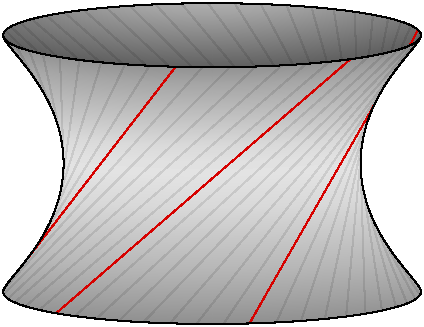
\includegraphics[height=2in]{main/Fig15-2-SinglyRuledHyperboloid-good}
\caption{Any three skew lines in space lie on a unique 
(and necessarily 
smooth) quadric surface, and all belong to the same 
ruling.
\index{ruling}%
}
\label{Fig15.2}
\end{figure}

\begin{enumerate}
\item Prove that $C$ lies on a unique quadric, and that $H^2(\sI_C) = 0$.
\index{quadric surface!containing three given lines}%
\item Compute the 
Hartshorne--Rao module
 $D(C)$.
\index{Hartshorne--Rao module}%
\item Show that if $\Gamma$ is the union of 3 points in $\PP^3$ then
$H^1\sI(\Gamma) = 0$ if and only~if the three points are collinear.
\item Using the exact sequence in cohomology coming from the short
exact sequence
$$
0\to \sI_C \ruto {\ \ell} \sI_C(1) \to \sI_\Gamma(1) \to 0 ,
$$
where $\ell$ is a linear form, show that the map of vector spaces
$$
H^1(\sI_C) \ruto {\ \ell} H^1(\sI_C(1))
$$
has rank $<2$ if and only~if $\ell$ vanishes on 3 collinear points on the
three lines (including the case when $\ell$ vanishes identically on one
of the lines).
Conclude that if a different union $C'$ of 3 skew lines is linked to $C$,
then $C'$ lies on the same quadric as $C$.
\end{enumerate}
See \cite{Migliore} for more examples of this type.
\end{exercise}

\begin{exercise}
Compute the 
Hilbert function
\index{Hilbert function}%
of the 
Hartshorne--Rao module
\index{Hartshorne--Rao module}%
 of a curve
of type $(a,b)$ on a smooth quadric surface.
\tohint{16.5}
\end{exercise}

\begin{exercise}[linkage addition \cite{Schwartau}]
\label{Liaison addition}
Suppose that $I, J$ are saturated ideals defining purely 1-dimensional
\index{linkage!addition}%
subschemes of $\PP^3$
and that $f,g$ is a regular sequence with $f\in I$ and $g\in J$.
Prove that $g I \cap fJ = (fg)$, and conclude that if $I,J$ are saturated
codimension 2 ideals
defining purely 1-dimensional schemes $C,C'$ in $\PP^3$
then $(gI+fJ)$ is a saturated ideal defining a purely 1-dimensional
scheme $C''$ with $D(C'') = D(C)(-\!\deg g) \oplus D(C')(-\!\deg f)$.
\tohint{16.6}
\end{exercise}

\begin{exercise}[basic double links]\label{Basic double links}
The special case of the construction in Exercise~\ref{Liaison addition}
\index{double links}%
in which $C'$ is trivial is already interesting.

\begin{enumerate}
\item Show that if $I$ is a 
saturated ideal of codimension 2
\index{saturated ideal}%
defining a purely 1-dimensional scheme $C$ in $\PP^3$
and $(f, g)$ is a regular sequence with $g\in I$,
then $fI+(g)$ defines a scheme $C'$ with $D(C') = D(C)(-\!\deg f)$.

\item Show directly that, with notation as above, $C'$ is directly
linked to $C$
in two steps. Since the degrees of the generators of $D(C')$ are more
positive, this
is sometimes called an \emph{ascending double link}. Geometrically it
amounts to taking the
union of $C$ with some	components that are 
complete intersections.
\index{complete intersection}%
\end{enumerate}
\end{exercise}

\begin{exercise}
\label{adjointness}
Here is a more general form of the last step in the proof of 
Proposition~\ref{similarities}(1). 
Suppose that $B\to A$ is a homomorphism
of rings, $X$ is an $A$-module and $Y$ is a
$B$-module. Show that there is a natural transformation
$$
\phi: \Hom_A(X, \Hom_B(A, Y)) \cong \Hom_B(X,Y)
$$
and that if $X = \Hom_B(A,Y)$, then the map
$$
A\to \Hom_A(\Hom_B(A,Y), \Hom_B(A, Y))
$$
taking an element $a\in A$ to multiplication by $a$ on the $A$-module
$\Hom_B(A, Y)$
is sent by $\phi$ to the evaluation map $\alpha \mapsto \alpha(a)$ for
$\alpha \in \Hom_B(A,Y)$.
\end{exercise}

\subsection*{Ropes and ribbons}
The simplest way to construct well-behaved nonreduced curves is
to take neighborhoods of smooth ones. Ropes and ribbons are examples of
this sort:


\begin{definition}
The \emph{rope defined from a curve $C \subset \PP^n$} is the scheme
$V(I^2_C)$ defined by the square of the ideal $C$.
\index{rope}%
\unif
\end{definition}

\begin{exercise}\label{hilbert function of rope}
If $C$ is the rope defined from a line $L\subset \PP^3$ then the Hilbert
function $h_C(m)$ and Hilbert polynomial $p_C(m)$ are both equal to
$3m+1$. Thus $C$ has degree 3 and
arithmetic genus 0. Note that the degree can also be computed as the
degree of
a general hyperplane section, since this is defined by the square of
the ideal of a point
in $\PP^2` `$.
\tohint{16.9}
\end{exercise}

\begin{exercise} To see why the rope in Exercise~\ref{hilbert function
of rope} should look like a twisted cubic, show that it is the flat
limit of a twisted cubic as follows:
Let $X \subset \PP^3$ be the twisted cubic with parametrization $x_i =
s^it^{3-i}$. Consider the one-parameter subgroup of $\PGL_4$ given in
homogeneous coordinates $x_0,\dots, x_3$ on $\PP^3$ by
$$
A_t : (x_0,\dots,x_3) \mapsto (tX_0, X_1, X_2,tX_3).
$$
Show that the 
flat limit,
\index{flat limit}%
 as $t\to 0$, of the 
\index{twisted cubic}%
twisted cubics
 $A_t(C)$
is the rope $V(X_0^2, X_0X_1,X_1^2)$.
\tohint{16.10}
\end{exercise}

\begin{exercise}\label{line and rope}
We saw in Section~\ref{LinkageIntro} that a twisted cubic curve is linked
to a line by the 
complete intersection of two quadrics.
\index{complete intersection!of two quadrics}%
Show that the same is true for the rope of
Exercise~\ref{hilbert function of rope}.
\end{exercise}

If $C$ is the rope defined from a line in $\PP^2` `$, then the Zariski
tangent space to $C$ at
any point is 2-dimensional; that is, it looks like a ribbon. More
generally:

\begin{definition}
By a \emph{ribbon} $X \subset \PP^n$ we mean a scheme of pure dimension~1
\index{ribbon}%
and multiplicity 2 whose support is a smooth, irreducible curve $C \subset
\PP^n$ and whose 
Zariski tangent space
\index{Zariski tangent space}%
 at every point is 2-dimensional
(Figure~\ref{Fig15.3}).
\begin{figure}
\vskip-5pt
\centerline {\includegraphics[width=2.4in]{"main/Fig15-3"}}
\vskip-8pt
\caption{A ribbon supported on a line.}
\label{Fig15.3}
\end{figure}
\end{definition}

\begin{exercise}
Suppose that $C\subset \PP^n$ is a ribbon. Show that $C$ is
contained in the rope defined from $C_{\mathrm{red}}$, and show that
the degree of $C$ is twice 
that
of $C_{\mathrm{red}}$.
\unskip\break %FMT
\null\hfill
\tohint{16.12}
\end{exercise}

\begin{exercise}
Unlike ropes, there are many different ribbons $C$ with the same smooth
curve $C_{\mathrm{red}}$,
and they can have different 
arithmetic genera.
\index{arithmetic genus}%
Suppose that $C\subset \PP^3$ is a ribbon such that $X = C_{\mathrm{red}}$
is the line $V(x_0,x_1)$.
Since $C$ is contained in the rope defined from $X$ we must have
$(x_0^2, x_0x_1,x_1^2) \subset I(C)$. The tangent space to $C$ at a
point $(0,0,s,t)$ meets the line $X' = V(x_2, x_3)$
at some point $(F(s,t),G(s,t),0,0)$, so $F$ and $G$ define a morphism
$\PP^1 \to \PP^1$;
thus they are homogeneous polynomials of the same degree $d$. It follows
that $I(C)$ also contains the element
$x_0 G(x_2, x_3) - x_1F(x_2,x_3)$. Show that the ideal of $C$ is obtained
by adding this form to the ideal of the rope, that is,
$$
I_C \; = \; \big(X_0^2, X_0X_1, X_1^2, F(X_3,X_4)X_0 + G(X_3,X_4)X_1\big)
.
$$
In case $d=1$, show that $C$ lies on a smooth quadric.
\end{exercise}

\subsection*{General adjunction}

The next two exercises illustrate Theorem~\ref{general adjunction}:

\begin{exercise}\label{codimension0}
Show that if $C\to D$ is a map of smooth curves with 
ramification index
\index{ramification!index}%
\index{adjunction}%
$e$ at $p\in C$, and $t$ is a local
analytic parameter at $p$, then
locally analytically at $p$ the sheaf $\sHom_C(\sO_C, \omega_D)$
is $\sO_C(e)$.
\end{exercise}

\begin{exercise}\label{codimension1}
Show that if $C\subset S$ is a
Cartier divisor
\index{Cartier divisor}%
on a surface $S$ with canonical sheaf $\omega_S$,
then $\sExt^1(\sO_C, \omega_S) \cong \sO_C\otimes \sO_S(C)$, and thus
$$K_C = (K_S+C)\cap C.$$
\index{linkage|)}%
\end{exercise}


